\scanpage{117}
\[
A'_0=\mathcal A'\qquad\pi_0(A)\text{ et }\pi_0(B)\text{ duaux}
\]
\[
\boxed{\begin{array}{l}
(3)\quad\left\{\begin{aligned}
H^1(K,A)&\simeq\underline{\operatorname{Ext}}_{k\mathrm{gr}}(\mathcal B,\mathbb Q/\mathbb Z)
\simeq\underline{\operatorname{Ext}}^1_{k\mathrm{gr}}(\mathcal B'{}^0,\mathbb Q/\mathbb Z)
\times\underline{\operatorname{Ext}}_{k\mathrm{gr}}(V,\mathbb Q/\mathbb Z)\\
H^1(K,B)&\simeq\underline{\operatorname{Ext}}_{k\mathrm{gr}}(\mathcal A,\mathbb Q/\mathbb Z)
\simeq\underline{\operatorname{Ext}}^1_{k\mathrm{gr}}(\mathcal A'{}^0,\mathbb Q/\mathbb Z)
\times\underline{\operatorname{Ext}}_{k\mathrm{gr}}(U,\mathbb Q/\mathbb Z)
\end{aligned}\right.\\[1em]
(2)\quad\pi_0(A)\text{ et }\pi_0(B)\text{ duaux (à valeurs dans }\mathbb Q/\mathbb Z)\\[1em]
(1)\quad0\longrightarrow\pi_1(A'_0)\longrightarrow
\end{array}}
\]
\margin{\deleted{\unsure{Vue d'ensemble}}}
\figure{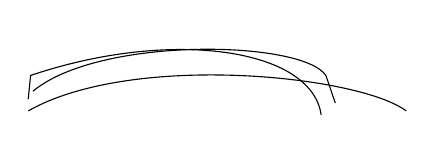
\begin{tikzpicture}[x=.6cm,y=.5cm]
\draw (0,0)--(.05,.6)..controls(3,1.8)and(6,1.3)..(6.2,-.4);
\draw (.1,.2)..controls(1.5,1.6)and(5.8,1.5)..(6.3,.6)--(6.5,-.1);
\draw (0,-.3)..controls(2.2,1.2)and(7,.6)..(8,-.3);
\end{tikzpicture}}
\figure{
\begin{tikzpicture}\draw (0,0)--(11,.2);\end{tikzpicture}}
\diagram{\begin{tikzcd}
0\arrow[r]&U\arrow[r]\arrow[d,phantom,"\text{unip. connexe}"]&
\mathcal A\arrow[r,dash]&\mathcal A'\arrow[r,dash]\arrow[d,phantom,"\text{sans unip. connexe}"]&0\\
&\phantom{U}&&\phantom{A'}&
\end{tikzcd}}
\[
\mu(A)=2\underbrace{\alpha(A^0)}_{\substack{\text{\unsure{composante}}\\\deleted{\text{multiplicative}}\\\text{abélienne}}}
+\underbrace{\mu(A^0)}_{\substack{\text{comp.}\\\text{multiplicative}}}
\]
\diagram{\begin{tikzcd}[column sep=small]
0\arrow[r,dash]&\operatorname{Ext}^1(\mathcal A'{}^0,\mathbb Q/\mathbb Z)\arrow[r]
\arrow[d,phantom,"(\mathbb Q/\mathbb Z)'{}^{\unsure{\mu(A)}}"]&
\operatorname{Ext}^1(\mathcal A,\mathbb Q/\mathbb Z)\arrow[r]\arrow[d,equal]&
\underline{\operatorname{Ext}}(U,\mathbb Q/\mathbb Z)\arrow[r]
\arrow[d,phantom,"\substack{\text{groupe \unsure{pro-algébrique}}\\\text{\unsure{unip.} connexe}}"]&0\\
&\phantom{X}&H^1(K,B)&\phantom{X}&
\end{tikzcd}}
\mspage{116}

